% Slide 41: Local Regression
\begin{frame}{رگرسیون محلی}{\lr{Local Regression}}
  \begin{columns}[T]
    \begin{column}{0.54\textwidth}
      \begin{itemize}
        \setlength{\itemsep}{6pt}
        \item \textbf{فرض اساسی:} مسائل غیرخطی در همسایگی‌های محلی کوچک تقریباً خطی هستند.
        \item \textbf{ایده اصلی:}
        \begin{itemize}
          \setlength{\itemsep}{4pt}
          \item برازش یک خط رگرسیون به صورت کاملاً محلی.
          \item انجام محاسبات صرفاً برای همان نقطه آزمون در زمان درخواست (\lr{Lazy Learning}).
        \end{itemize}
      \end{itemize}
    \end{column}
    \begin{column}{0.44\textwidth}
      \begin{center}
        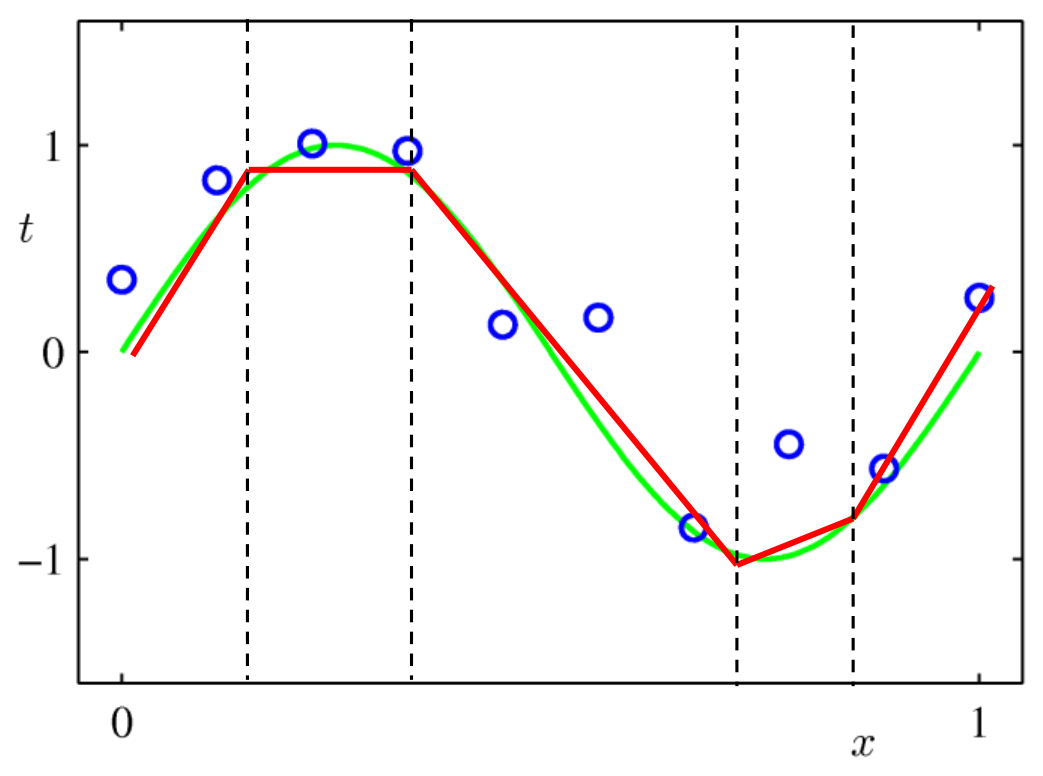
\includegraphics[width=\textwidth,height=4.2cm,keepaspectratio]{images/slide41_local_regression_weights.png}
      \end{center}
    \end{column}
  \end{columns}
\end{frame}

% Slide 42: Local Regression Steps
\begin{frame}{گام‌های رگرسیون محلی}{\lr{Local Regression Algorithm (KNN + Linear Regression)}}
  \begin{columns}[T]
    \begin{column}{0.54\textwidth}
      \begin{itemize}
        \setlength{\itemsep}{5pt}
        \item ترکیبی هوشمندانه از $k$ نزدیک‌ترین همسایه و رگرسیون خطی:
        \begin{enumerate}
          \setlength{\itemsep}{4pt}
          \item برای نقطه ورودی جدید، $k$ همسایه نزدیک‌تر را بازیابی کن.
          \item یک مدل رگرسیون خطی محلی فقط روی این $k$ همسایه آموزش بده.
          \item با استفاده از مدل محلی، مقدار $y$ را برای نقطه ورودی تخمین بزن.
        \end{enumerate}
      \end{itemize}
    \end{column}
    \begin{column}{0.44\textwidth}
      \begin{center}
        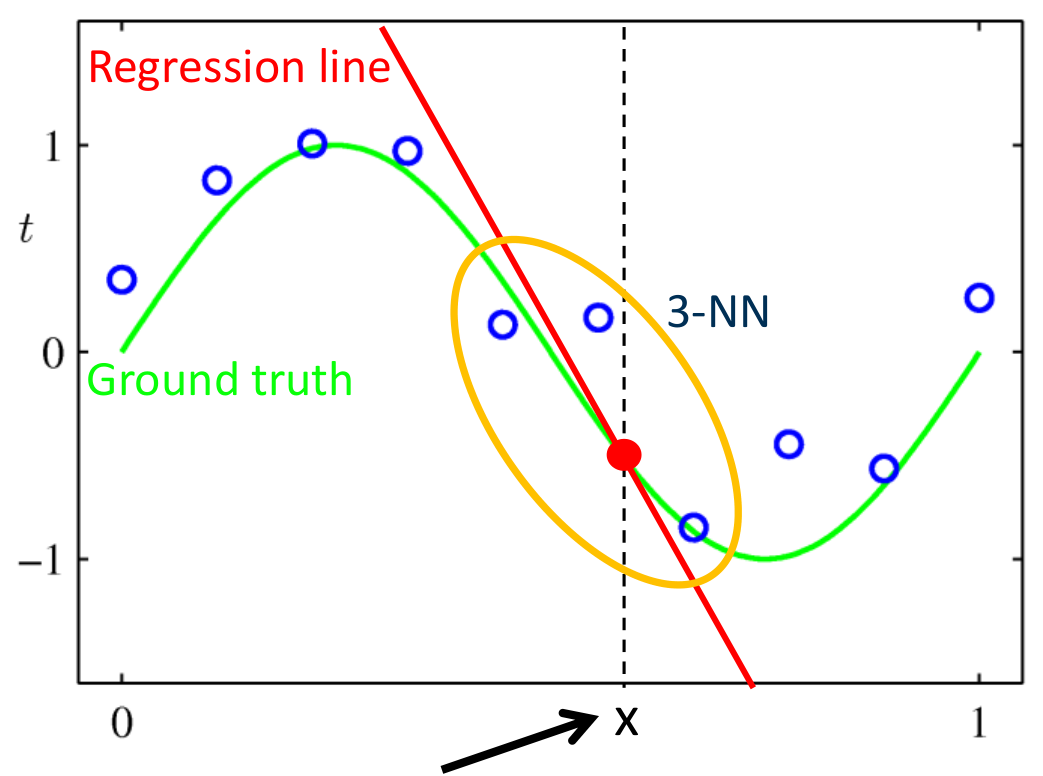
\includegraphics[width=\textwidth,height=4.2cm,keepaspectratio]{images/slide42_local_regression_tangents.png}
      \end{center}
    \end{column}
  \end{columns}
\end{frame}

% Slide 43: Discussion of Local Regression
\begin{frame}{مزایا و معایب رگرسیون محلی}{\lr{Discussion of Local Regression}}
  \begin{itemize}
    \setlength{\itemsep}{6pt}
    \item \textbf{مزایا:}
    \begin{itemize}
      \setlength{\itemsep}{4pt}
      \item انطباق بسیار عالی بر الگوها و روندهای غیرخطی پیچیده.
      \item تقریب محلی بسیار دقیق‌تر از میانگین‌گیری ساده در رگرسیون $k$-NN.
    \end{itemize}
    \item \textbf{معایب و چالش‌ها:}
    \begin{itemize}
      \setlength{\itemsep}{4pt}
      \item \textbf{هزینه محاسباتی بالا در زمان پیش‌بینی:} \lr{(Slow at runtime)}
      به ازای هر نمونه آزمون، باید نزدیک‌ترین همسایه‌ها جستجو شده و یک مدل خطی از نو حل شود!
    \end{itemize}
  \end{itemize}
\end{frame}

% Slide 44: ANNs for Classification Recap
\begin{frame}{شبکه‌های عصبی برای رگرسیون: یادآوری طبقه‌بندی}{\lr{ANNs: Recap for Classification}}
  \begin{itemize}\setlength{\itemsep}{3pt}\small
    \item \textbf{یادآوری:} چگونه از شبکه‌های عصبی در طبقه‌بندی استفاده کردیم؟
  \end{itemize}
  \vspace{-0.1cm}
  \begin{columns}[c]
    \begin{column}{0.48\textwidth}
      \centering
      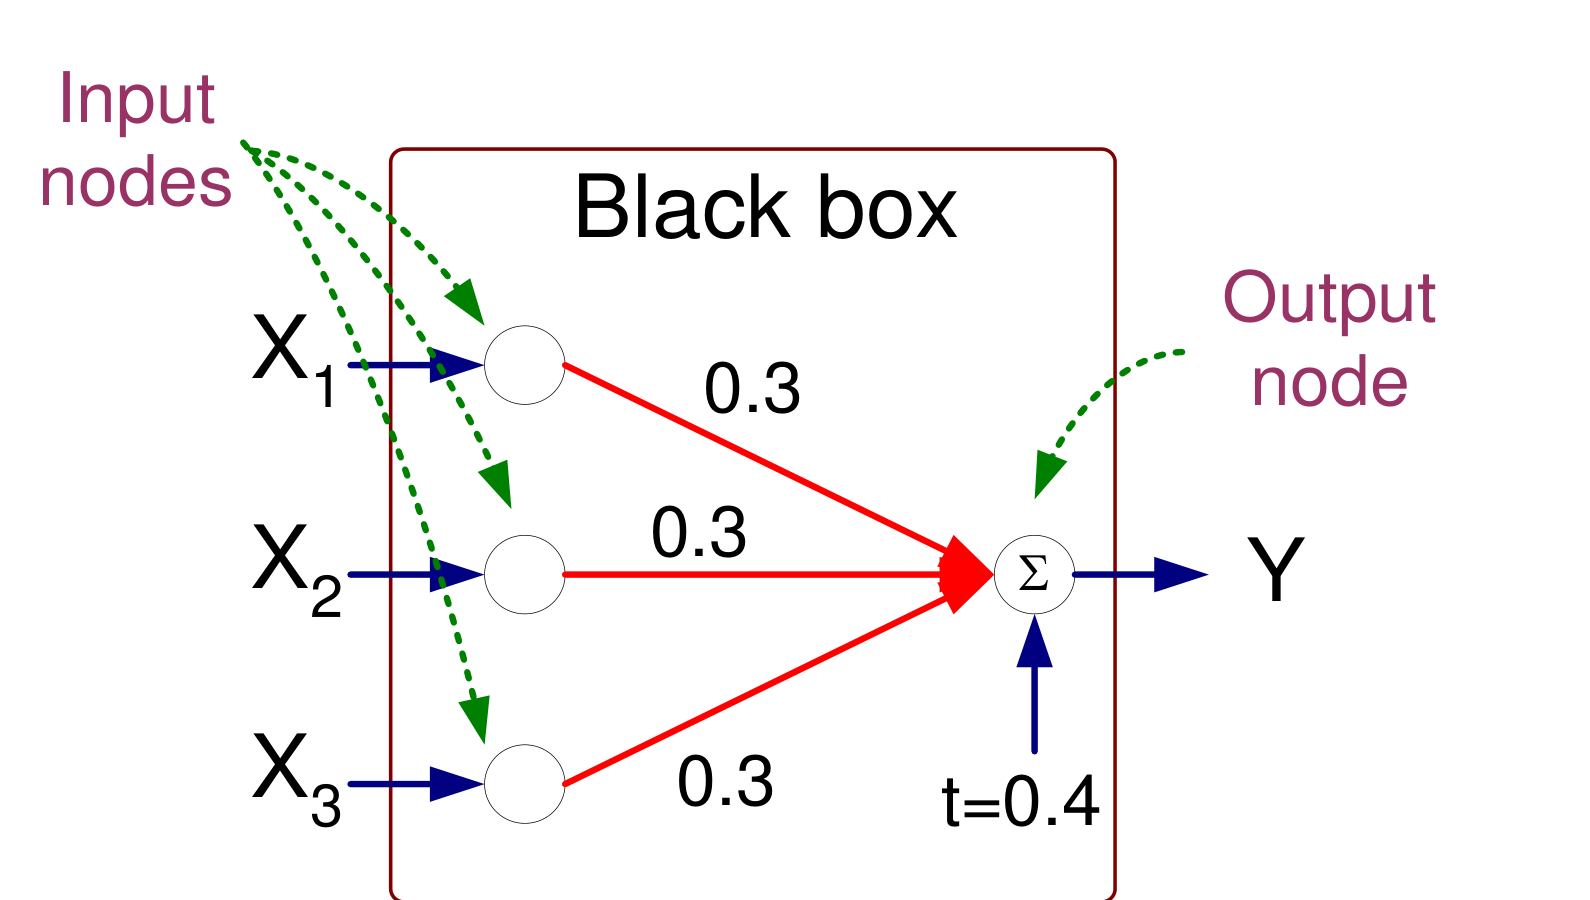
\includegraphics[height=2.8cm,keepaspectratio]{images/slide44_black_box.png}
    \end{column}
    \begin{column}{0.48\textwidth}
      \centering
      {\fontsize{7.5}{9}\selectfont
      \begin{tabular}{|cccc|}
        \hline
        $X_1$ & $X_2$ & $X_3$ & $Y$ \\ \hline
        1 & 0 & 0 & 0 \\
        1 & 0 & 1 & 1 \\
        1 & 1 & 0 & 1 \\
        1 & 1 & 1 & 1 \\
        0 & 0 & 1 & 0 \\
        0 & 1 & 0 & 0 \\
        0 & 1 & 1 & 1 \\
        0 & 0 & 0 & 0 \\ \hline
      \end{tabular}
      }
    \end{column}
  \end{columns}
  \vspace{0.15cm}
  \par\noindent\makebox[\linewidth][c]{$\displaystyle Y = I(0.3 X_1 + 0.3 X_2 + 0.3 X_3 - 0.4 > 0)$}\par\vspace{2pt}
  \par\noindent\makebox[\linewidth][c]{$\displaystyle \text{\rl{که در آن:}}\quad I(z) = \begin{cases} 1 & \text{\rl{اگر $z$ درست باشد}} \\ 0 & \text{\rl{در غیر این صورت}} \end{cases}$}\par
\end{frame}

% Slide 45: ANNs Continuous Prediction
\begin{frame}{شبکه‌های عصبی: خروجی پیوسته رگرسیون}{\lr{ANNs: Continuous Output Prediction}}
  \begin{itemize}\setlength{\itemsep}{3pt}\small
    \item تابع $I(z)$ برای تفکیک دو کلاس به کار می‌رفت:
    \par\vspace{1pt}\noindent\makebox[\linewidth][c]{$\displaystyle Y = I(0.3 X_1 + 0.3 X_2 + 0.3 X_3 - 0.4 > 0)$}\par\vspace{1pt}
    \par\noindent\makebox[\linewidth][c]{$\displaystyle \text{\rl{که در آن:}}\quad I(z) = \begin{cases} 1 & \text{\rl{اگر $z$ درست باشد}} \\ 0 & \text{\rl{در غیر این صورت}} \end{cases}$}\par\vspace{4pt}
    \item با این حال، می‌توانیم به سادگی از \textbf{ترکیب خطی درونی} برای پیش‌بینی یک مقدار عددی پیوسته (بین ۰ و ۱) استفاده کنیم:
    \par\vspace{2pt}\noindent\makebox[\linewidth][c]{$\displaystyle \hat{Y} = 0.3 X_1 + 0.3 X_2 + 0.3 X_3 - 0.4$}\par\vspace{2pt}
    \begin{itemize}\footnotesize
      \item خروجی این فرمول یک عدد حقیقی پیوسته بدون محدودیت کلاس است.
    \end{itemize}
  \end{itemize}
\end{frame}

% Slide 46: What has changed
\begin{frame}{تغییرات شبکه عصبی در حالت رگرسیون}{\lr{ANNs: What Has Changed for Regression?}}
  \begin{itemize}
    \setlength{\itemsep}{6pt}
    \item \textbf{تابع فعال‌سازی لایه خروجی:}
    عدم استفاده از حد آستانه یا سیگموئید در گره نهایی؛ خروجی به شکل تابع همانی (\lr{Identity / Linear}) باقی می‌ماند.
    \item \textbf{داده‌های آموزش:}
    بردار متغیرهای ورودی به همراه یک متغیر هدف \textbf{پیوسته عددی} (به جای برچسب گسسته کلاس).
    \item \textbf{تابع خطا و یادگیری:}
    به جای خطای طبقه‌بندی یا آنتروپی متقاطع، از \textbf{میانگین مربعات خطا (\lr{MSE})} به عنوان تابع هزینه استفاده می‌شود.
  \end{itemize}
\end{frame}

% Slide 47: Multi-Layer Perceptron Regression
\begin{frame}{شبکه‌های عصبی چندلایه برای رگرسیون غیرخطی}{\lr{Multi-Layer Neural Networks for Regression}}
  \begin{columns}[T]
    \begin{column}{0.54\textwidth}
      \begin{itemize}
        \setlength{\itemsep}{5pt}
        \item با یک تک‌نورون فقط می‌توان مدل‌های خطی را برازش کرد (ترکیب خطی متغیرهای ورودی).
        \item \textbf{حل مسائل پیچیده غیرخطی:}
        \begin{itemize}
          \setlength{\itemsep}{3pt}
          \item افزودن \textbf{لایه‌های پنهان (\lr{Hidden Layers})} با توابع فعال‌سازی غیرخطی (\lr{ReLU}، \lr{Sigmoid}).
          \item قضیه تقریب عام: قابلیت یادگیری و تقریب هر تابع پیوسته دلخواه!
        \end{itemize}
      \end{itemize}
    \end{column}
    \begin{column}{0.44\textwidth}
      \begin{center}
        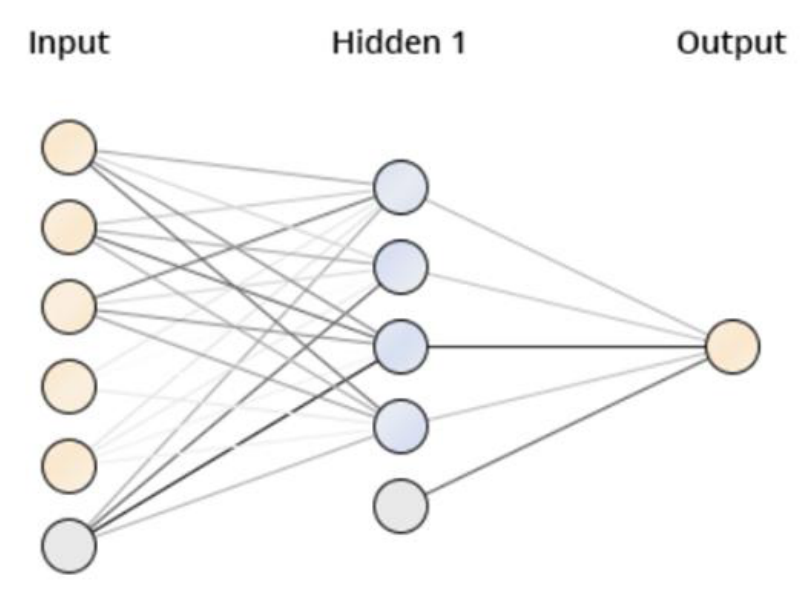
\includegraphics[width=\textwidth,height=3.8cm,keepaspectratio]{images/slide47_ann_mlp_regression.png}
      \end{center}
    \end{column}
  \end{columns}
\end{frame}

% Slide 48: Bias-Variance Tradeoff
\begin{frame}{موازنه بایاس و واریانس}{\lr{The Bias/Variance-Tradeoff}}
  \begin{itemize}
    \setlength{\itemsep}{4pt}
    \item هدف ما یادگیری مدل‌هایی با قابلیت تعمیم بالا (\lr{Generalization}) به داده‌های نادیده است.
    \item خطای تعمیم هر مدل از مجموع \textbf{سه مؤلفه اساسی} تشکیل شده است:
    \par\vspace{2pt}\noindent\makebox[\linewidth][c]{$\displaystyle \mathbb{E}[(y - \hat{f}(x))^2] = \text{Bias}[\hat{f}(x)]^2 + \text{Var}[\hat{f}(x)] + \sigma^2$}\par\vspace{2pt}
    \begin{itemize}
      \setlength{\itemsep}{3pt}
      \item \textbf{بایاس یا اریبی} (\lr{Bias}): ناشی از فرض‌های ساده‌انگارانه مدل (کم‌برازش مدل‌های بسیار ساده).
      \item \textbf{واریانس} (\lr{Variance}): ناشی از حساسیت بیش‌ازحد مدل به نوسانات کوچک داده‌های آموزش (بیش‌برازش مدل‌های بسیار منعطف).
      \item \textbf{خطای کاهش‌ناپذیر} ($\sigma^2$ - \lr{Irreducible Error}): نوفه ذاتی داده‌ها (تنها با پالایش سنسورها و پاکسازی داده‌ها کم می‌شود).
    \end{itemize}
  \end{itemize}
\end{frame}

% Slide 49: Tradeoff Curve & Flexibility
\begin{frame}{انعطاف‌پذیری مدل و منحنی موازنه}{\lr{Model Flexibility and the Tradeoff Curve}}
  \begin{itemize}
    \item سه مدل با انعطاف‌پذیری متفاوت برای برازش یک تابع:
  \end{itemize}
  \vspace{-0.1cm}
  \begin{center}
    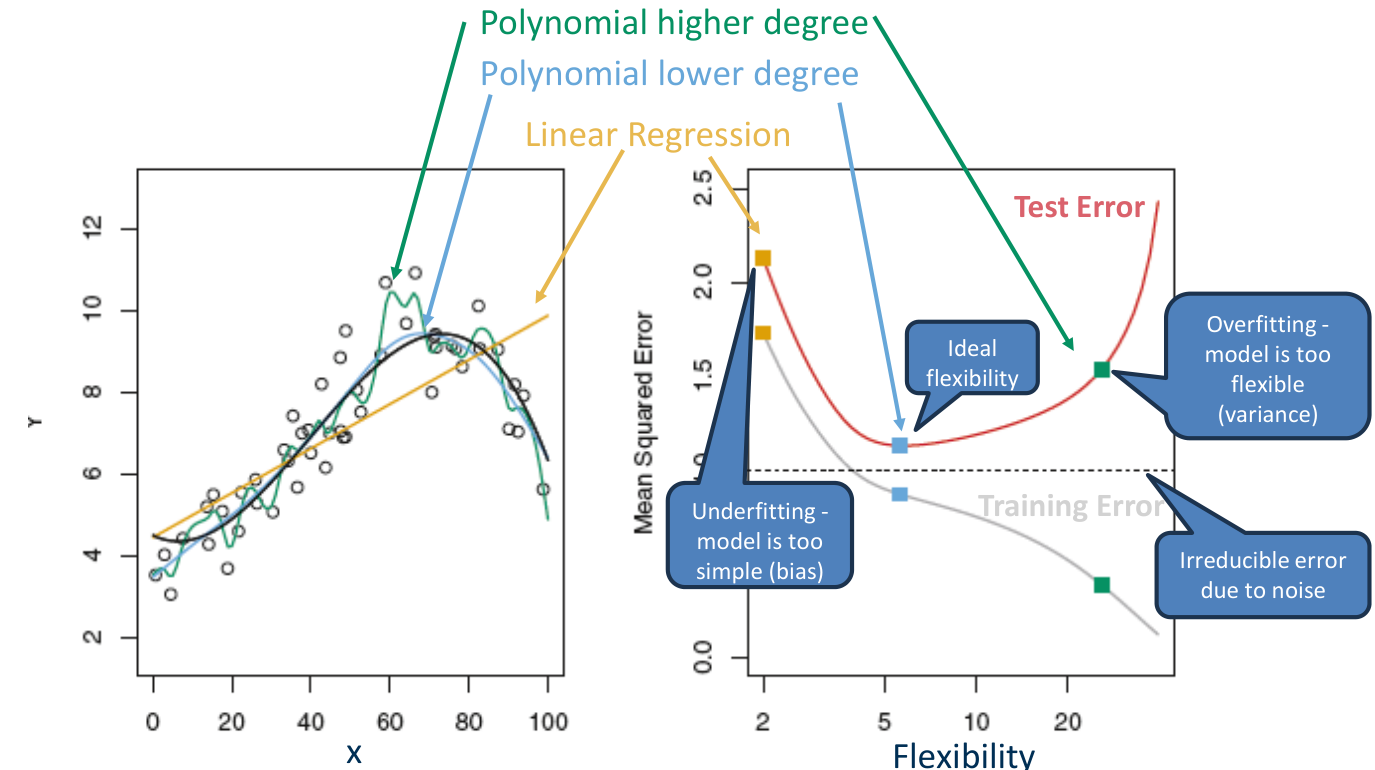
\includegraphics[width=0.96\textwidth,height=4.4cm,keepaspectratio]{images/slide49_bias_variance_models.png}
  \end{center}
\end{frame}

% Slide 50: Learning Method & Hyperparameter Selection
\begin{frame}{یافتن انعطاف‌پذیری بهینه}{\lr{Selecting Method \& Hyperparameters}}
  \begin{columns}[T]
    \begin{column}{0.58\textwidth}
      \begin{itemize}
        \setlength{\itemsep}{4pt}
        \item \textbf{یافتن نقطه تعادل بهینه بایاس و واریانس با:}
        \begin{itemize}
          \item آزمودن الگوریتم‌های یادگیری مختلف (خطی، چندجمله‌ای، درخت تصمیم، شبکه‌های عصبی).
          \item تنظیم فراپارامترها (درجه چندجمله‌ای، ضریب جریمه ریج، عمق درخت، لایه‌های پنهان).
        \end{itemize}
        \item \textbf{سه راهکار دیگر برای بهبود مدل:}
        \begin{itemize}
          \item افزایش حجم داده‌های آموزش (\lr{More Data})
          \item افزودن موارد حدی چالش‌برانگیز (\lr{Corner Cases})
          \item پاکسازی نوفه از داده‌های آموزش (\lr{Data Cleansing})
        \end{itemize}
      \end{itemize}
    \end{column}
    \begin{column}{0.40\textwidth}
      \begin{center}
        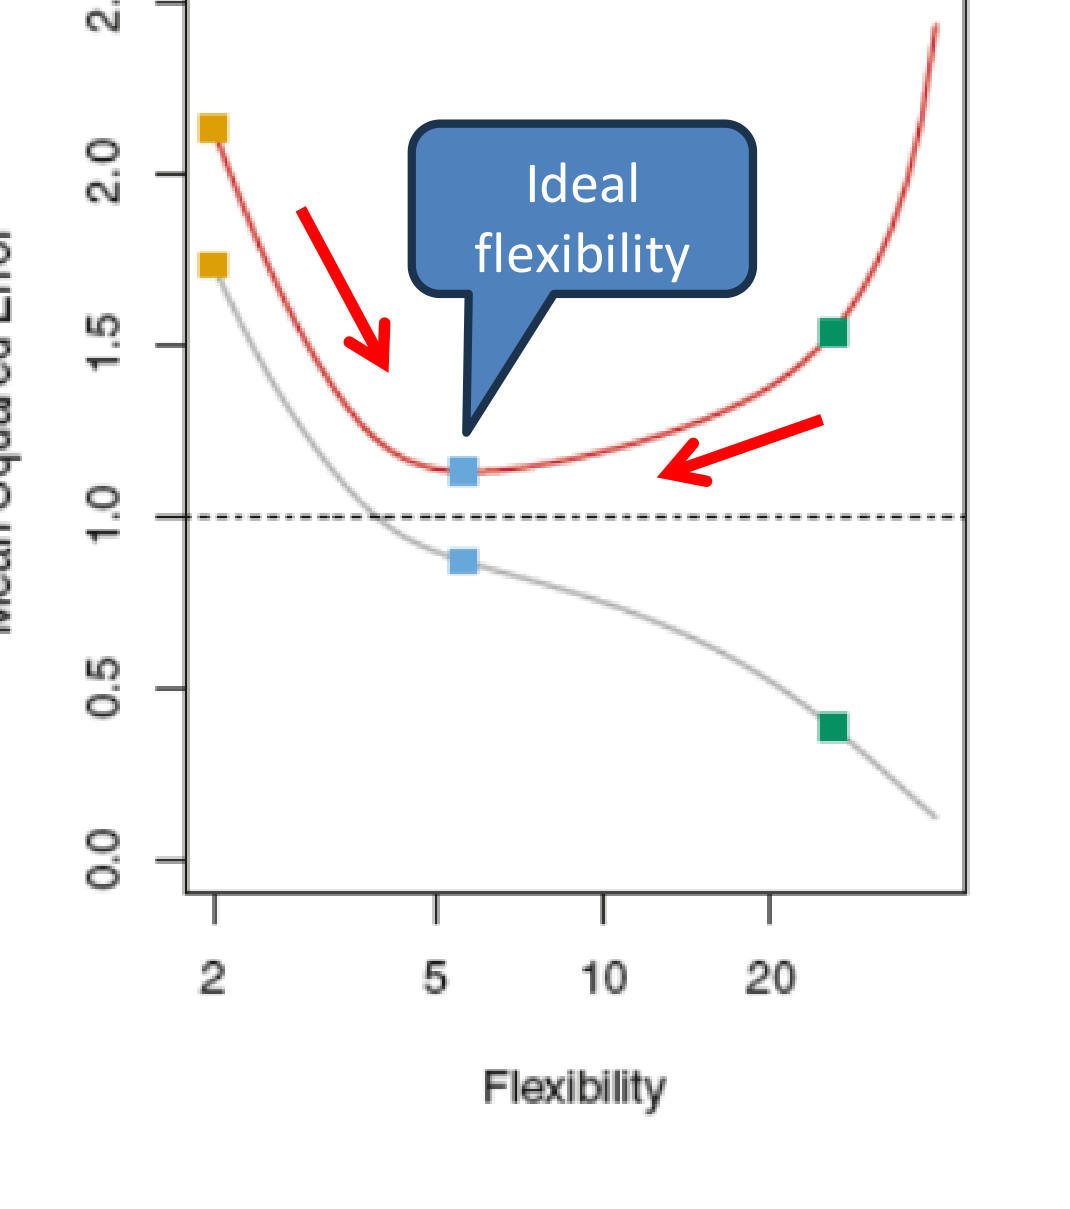
\includegraphics[width=\textwidth,height=4.2cm,keepaspectratio]{images/slide50_flexibility_tuning_curve.png}
      \end{center}
    \end{column}
  \end{columns}
\end{frame}

% Slide 51: Learning Curves
\begin{frame}{منحنی‌های یادگیری در کم‌برازش و بیش‌برازش}{\lr{Learning Curves for Under- and Overfitting Models}}
  \begin{itemize}
    \setlength{\itemsep}{3pt}
    \item تجسم خطای آموزش و خطای آزمون برای اندازه‌های مختلف مجموعه‌های آموزش:
    \begin{itemize}
      \item در مدل‌های بیش‌برازش، شکاف میان خطای آموزش و آزمون با افزودن داده‌های بیشتر کاهش می‌یابد.
      \item دسترسی به داده‌های بیشتر به ما اجازه استفاده از مدل‌های منعطف‌تر (نظیر یادگیری عمیق) را می‌دهد.
    \end{itemize}
  \end{itemize}
  \vspace{0.1cm}
  \begin{center}
    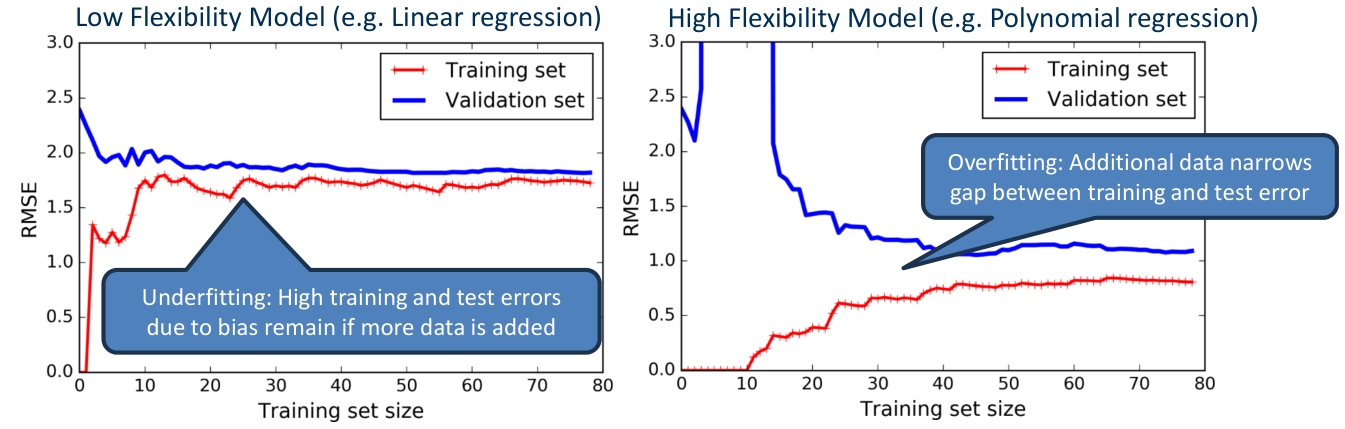
\includegraphics[width=0.96\textwidth,height=3.4cm,keepaspectratio]{images/slide51_learning_curves_under_overfit.png}
  \end{center}
\end{frame}

% Slide 52: Classification to Regression and Back
\begin{frame}{تبدیل دوطرفه طبقه‌بندی و رگرسیون}{\lr{From Classification to Regression and Back}}
  \begin{itemize}
    \setlength{\itemsep}{5pt}
    \item ابتدا با طبقه‌بندی آشنا شدیم و پرسیدیم چگونه می‌توان از طبقه‌بندی به رگرسیون رسید؟
    \item \textbf{پرسش معکوس:} آیا می‌توان از الگوریتم‌های رگرسیون برای طبقه‌بندی استفاده نمود؟
    \item \textbf{رویکرد تبدیل:}
    \begin{itemize}
      \setlength{\itemsep}{3pt}
      \item برای طبقه‌بندی دودویی: کدگذاری مثبت به عنوان $1.0$ و منفی به عنوان $0.0$.
      \item یادگیری مدل رگرسیون بر روی این مقادیر عددی.
      \item پیش‌بینی کلاس منفی برای بازه \lr{$(-\infty, 0.5]$} و مثبت برای بازه \lr{$(0.5, \infty)$}.
    \end{itemize}
    \item به طور مشابه برای داده‌های ترتیبی (\lr{Ordinal}) نظیر ضعیف/متوسط/خوب.
    \item مسائل چندکلاسه غیرترتیبی پیچیده‌تر بوده و نیازمند رویکرد یک‌در-برابر-همه (\lr{One-vs-Rest}) هستند.
  \end{itemize}
\end{frame}
